% appendix.tex -- appendix sections of paper.tex, \input{} after the \appendix counter lines.
% Hand-written like paper.tex; the tables it \input{}s under tables/ are GENERATED by main.R
% (build_paper_tables() + export_paper_tables()) and are never edited by hand. Paths are
% relative to paper/, where the document compiles.

%======================================================================
\section{Data and sample details}\label{sec:app-data}
%======================================================================

\paragraph{Hours coding.}
The CBS records usual weekly hours in bins; each bin is assigned its median ($4$, $11$, $18$,
$25.5$, $32$, $37$, $42$, $47$, $54.5$ and $78.5$ hours) and the two irregular-hours codes are
imputed from observed medians within the same period. Mid-distribution bins are about five hours
wide, so an effect smaller than one bin width, such as the headline estimate, is best read as a
shift in the share of women crossing a bin boundary. In the 2017 file, employed respondents
absent from work in the reference week had their usual hours recorded as zero, whereas from 2018
onward the same respondents were assigned a real value; left uncorrected, this enters the
pre-period as roughly $5{,}200$ spurious zeros, and because absence is more common among mothers
($12.4\%$ of employed mothers against $7.3\%$ of childless women) they fall unevenly across the
comparison the paper makes. Defining hours on the reference-week workers in \emph{every} year
costs about $10\%$ of each year's employed sample, makes the hours population identical across
years, and narrows the estimand to usual hours among women who were working.

\paragraph{Reference-week absence and exposure.}
Absence is related to exposure. Among employed women with a matched occupation, by the quartiles
of Figure~\ref{fig:dose-response}, the absence shares are $14.4\%$, $8.5\%$, $9.5\%$ and $9.6\%$.
Among mothers the top-quartile share fell from $12.1\%$ to $10.4\%$ after 2021 and the
bottom-quartile share rose from $15.5\%$ to $16.9\%$; among childless women the top-quartile
share is $6.1\%$ in both periods. Movement across the absence margin is therefore part of what
selection into the observed-hours sample means, which is why the bounds of
Appendix~\ref{sec:app-lee} define selection on that sample.

\paragraph{Panel structure.}
The survey is a rotating panel. The $258{,}175$ reference-week workers of
Table~\ref{tab:descriptives} come from $64{,}602$ distinct respondents, about four observations
each and two to three within a single survey year, with $96\%$ of rows belonging to someone who
appears more than once; the regressions use $251{,}857$ of those rows from $63{,}199$
respondents, the difference being the $6{,}318$ rows whose education code is missing (education
is the only control with missing values). Treating the observations as independent would
understate standard errors by a factor of roughly $1.8$, which is why every DiD and every
descriptive interval is clustered by individual. The panel does not support within-person
identification: of the $80{,}560$ women in the full sample, $1.9\%$ are interviewed on both sides
of the pre/post boundary, so an individual fixed-effects design was considered and rejected.
% Provenance: 1,514 of 80,560 distinct individuals (1.88%) appear in both the pre- and post-period
% (check_idpuf_panel_structure(), scripts/validation.R). The 6,318 rows with a missing education
% code (TeudaGvoha 99 -> NA) are the only listwise deletions: confirmed on cleaned_df.rds,
% 2026-09-23, with zero NAs in the other four controls on the hours sample.

\paragraph{Hours year by year.}
Panel~(a) of Figure~\ref{fig:hours-by-year} unpools the pre-period. The raw mother-minus-non-mother gap is
$-1.37$ hours in 2017, $-1.48$ in 2018 and $-1.67$ in 2019, three years within a third of an hour
of each other and each within the others' confidence bounds: the groups were not diverging before
treatment. The post-period path is $-1.37$, $-1.53$ and $-0.80$, not monotone and not
individually distinguishable, so the timing reading in the Discussion rests on the event studies
of Figure~\ref{fig:pretrend}, not on this series.

\paragraph{Commuting.}
Mothers were the \emph{more} mobile group in every year, working outside their locality of
residence $48.2\%$ of the time in 2019 against $46.1\%$ of childless women, and their commuting
fell less in 2021 ($1.5$ against $3.9$ percentage points, a difference of $2.39$ points,
SE $1.17$). This is consistent with remote work relaxing a time constraint for women who were
already commuting; it is descriptive evidence only, and no specification uses locality of work as
an outcome.

%======================================================================
\section{Exposure construction}\label{sec:appendix-exposure}
%======================================================================

\paragraph{The external score.}
The \citet{dingel2020} teleworkability score reaches the two-digit ISCO-08 level through an
O*NET/SOC-to-ISCO crosswalk. Teaching (ISCO 23) is the clearest case of a US task-based score
misclassifying Israeli practice: it scores $0.966$ on the external index, yet Israeli schools,
closed and reopened in stages through 2020 and early 2021 \citep{somekh2021, hale2021}, were fully
in person throughout the 2022--23 survey years, and teachers did not work from home. The
crosswalk that maps the US occupation codes onto ISCO-08 is not documented in the replication
materials, so a reader can check the forty resulting scores (Table~\ref{tab:exposure-scores}) but
not rebuild them from the source.

\paragraph{The calibration rule.}
The external score is replaced by the realized 2022--23 Israeli WFH share only where the gap
between the two is large (greater than $0.5$) \emph{and} distinguishable from sampling noise by a
one-sided test at the 95\% level with a standard error clustered by individual. Ten of the forty
two-digit occupations are swapped: teaching falls from $0.966$ to $0.069$, clerical support
(ISCO 41) from $1.000$ to $0.098$, ICT professionals (ISCO 25) from $1.000$ to $0.360$. The
realized shares are computed on men and women together; Table~\ref{tab:robust} re-derives them
from men alone. The realized index used as a bound is the realized Israeli WFH share by
occupation, anchored to 2021 (no 2020 extract exists) with a minimum of 200 observations per
occupation.

\paragraph{Fit.}
Across the forty occupations, on men and women pooled over 2021--23, the calibrated score has a
correlation of $0.53$ with the share who worked from home in the reference week and an
occupation-size-weighted slope of $0.40$ (SE $0.09$), so it is relevant. The raw external index
fits better in levels (correlation $0.74$), because swapping ten occupations onto realized shares
while leaving thirty on task-based probabilities mixes two scales. The calibration's contribution
is not a better cross-sectional fit but the removal of ten grossly mis-scored occupations from the
treated tail. Table~\ref{tab:exposure-scores} lists, for each occupation, the external score, the
realized 2022--23 share the calibration tests it against, whether the score was swapped, the
calibrated score the hours DDD uses, and the realized reference-week share over 2021--23;
panel~(b) of Figure~\ref{fig:first-stage} plots the last against the calibrated score.

\begin{table}[htbp]
\centering
\begin{threeparttable}
\caption{External, realized and calibrated WFH exposure by two-digit occupation}\label{tab:exposure-scores}
\renewcommand{\baselinestretch}{1}\scriptsize
\setlength{\tabcolsep}{3pt}
\begin{tabular}{lp{5.2cm}cccccc}
\toprule
ISCO & Occupation (ISCO-08 sub-major group) & Ext. & Real.\ 22--23 & Swap & Calib. & Ref.-wk 21--23 & $N$ \\
\midrule
11 & Chief executives and legislators & 0.900 & 0.155 & yes & 0.155 & 0.320 & 2{,}855 \\
12 & Administrative and commercial managers & 0.892 & 0.143 & yes & 0.143 & 0.336 & 3{,}859 \\
13 & Production and specialised services managers & 0.638 & 0.097 & yes & 0.097 & 0.199 & 9{,}990 \\
14 & Hospitality, retail and other services managers & 0.773 & 0.066 & yes & 0.066 & 0.132 & 2{,}827 \\
21 & Science and engineering professionals & 0.644 & 0.210 &  & 0.644 & 0.349 & 13{,}228 \\
22 & Health professionals & 0.101 & 0.059 &  & 0.101 & 0.088 & 9{,}665 \\
23 & Teaching professionals & 0.966 & 0.069 & yes & 0.069 & 0.184 & 20{,}496 \\
24 & Business and administration professionals & 0.943 & 0.233 & yes & 0.233 & 0.449 & 10{,}479 \\
25 & ICT professionals & 1.000 & 0.360 & yes & 0.360 & 0.615 & 14{,}638 \\
26 & Legal, social and cultural professionals & 0.678 & 0.215 &  & 0.678 & 0.371 & 13{,}344 \\
31 & Science and engineering associate professionals & 0.144 & 0.059 &  & 0.144 & 0.106 & 3{,}926 \\
32 & Health associate professionals & 0.057 & 0.080 &  & 0.057 & 0.084 & 2{,}203 \\
33 & Business and administration associate professionals & 0.684 & 0.123 & yes & 0.123 & 0.223 & 22{,}415 \\
34 & Legal, social and cultural associate professionals & 0.577 & 0.142 &  & 0.577 & 0.206 & 5{,}480 \\
35 & ICT technicians & 0.750 & 0.244 &  & 0.750 & 0.380 & 2{,}491 \\
41 & General and keyboard clerks & 1.000 & 0.098 & yes & 0.098 & 0.144 & 4{,}846 \\
42 & Customer services clerks & 0.292 & 0.096 &  & 0.292 & 0.159 & 3{,}875 \\
43 & Numerical and material recording clerks & 0.526 & 0.071 &  & 0.526 & 0.152 & 4{,}948 \\
44 & Other clerical support workers & 0.625 & 0.083 & yes & 0.083 & 0.161 & 1{,}049 \\
51 & Personal service workers & 0.271 & 0.146 &  & 0.271 & 0.144 & 7{,}808 \\
52 & Sales workers & 0.200 & 0.050 &  & 0.200 & 0.063 & 8{,}704 \\
53 & Personal care workers & 0.300 & 0.046 &  & 0.300 & 0.045 & 17{,}206 \\
54 & Protective services workers & 0.100 & 0.008 &  & 0.100 & 0.011 & 3{,}969 \\
61 & Market-oriented skilled agricultural workers & 0.182 & 0.027 &  & 0.182 & 0.051 & 1{,}325 \\
62 & Market-oriented skilled forestry, fishery and hunting workers & 0.179 & 0.000 &  & 0.179 & 0.045 & 22 \\
63 & Subsistence farmers, fishers, hunters and gatherers & 0.000 & 0.375 &  & 0.000 & 0.375 & 8 \\
71 & Building and related trades workers & 0.027 & 0.008 &  & 0.027 & 0.016 & 5{,}208 \\
72 & Metal, machinery and related trades workers & 0.000 & 0.008 &  & 0.000 & 0.013 & 3{,}982 \\
73 & Handicraft and printing workers & 0.138 & 0.118 &  & 0.138 & 0.129 & 666 \\
74 & Electrical and electronic trades workers & 0.000 & 0.022 &  & 0.000 & 0.042 & 3{,}424 \\
75 & Food, wood, garment and other craft workers & 0.073 & 0.122 &  & 0.073 & 0.109 & 2{,}304 \\
81 & Stationary plant and machine operators & 0.000 & 0.019 &  & 0.000 & 0.017 & 2{,}407 \\
82 & Assemblers & 0.000 & 0.012 &  & 0.000 & 0.015 & 1{,}166 \\
83 & Drivers and mobile plant operators & 0.237 & 0.006 &  & 0.237 & 0.006 & 8{,}480 \\
91 & Cleaners and helpers & 0.000 & 0.004 &  & 0.000 & 0.003 & 3{,}474 \\
92 & Agricultural, forestry and fishery labourers & 0.000 & 0.007 &  & 0.000 & 0.016 & 192 \\
93 & Labourers in mining, construction, manufacturing and transport & 0.120 & 0.006 &  & 0.120 & 0.008 & 2{,}659 \\
94 & Food preparation assistants & 0.000 & 0.013 &  & 0.000 & 0.011 & 649 \\
95 & Street and related sales and service workers & 0.000 & 0.000 &  & 0.000 & 0.043 & 23 \\
96 & Refuse workers and other elementary workers & 0.250 & 0.022 &  & 0.250 & 0.024 & 493 \\
\bottomrule
\end{tabular}

\begin{tablenotes}\footnotesize
\item Ext.: the \citet{dingel2020} teleworkability score at the two-digit ISCO-08 level, via
the crosswalk described above. Real.\ 22--23: share of employed
respondents (men and women, all ages in the extract) who usually work from home in 2022--23,
the calibration's benchmark; Swap: the calibration replaced the external score with it.
Calib.: the score the hours DDD uses. Ref.-wk 21--23: share who worked from home in the survey
reference week over 2021--23, men and women pooled, with $N$ the pooled employed sample carrying
that item. Codes 1--3 (armed forces) carry no external score and are not in the sample.
\end{tablenotes}
\end{threeparttable}
\end{table}

\begin{figure}[htbp]
\centering
\begin{minipage}[t]{0.44\textwidth}\centering
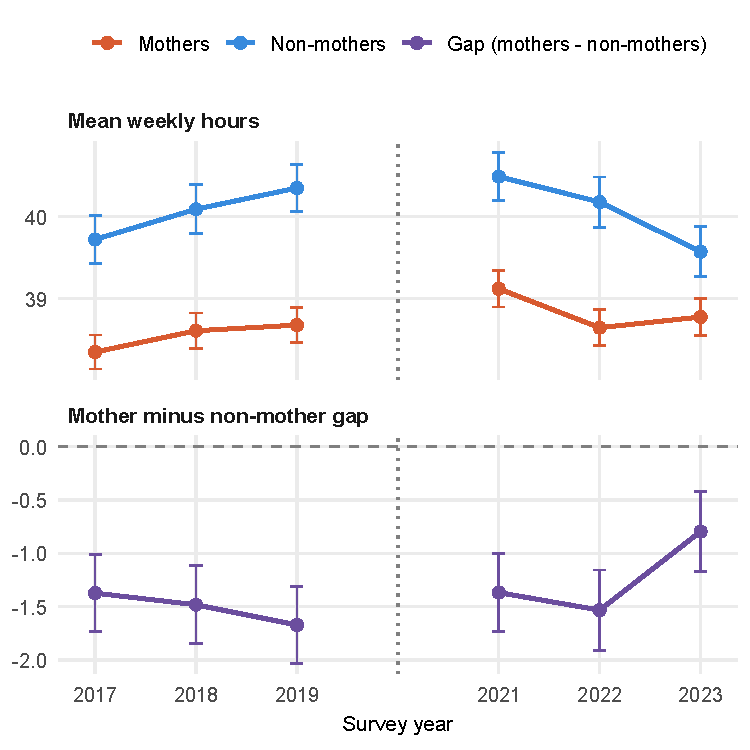
\includegraphics[width=\linewidth]{../outputs/figures/hours_by_year.pdf}\\
{\small (a) Weekly hours by survey year}
\end{minipage}\hfill
\begin{minipage}[t]{0.52\textwidth}\centering
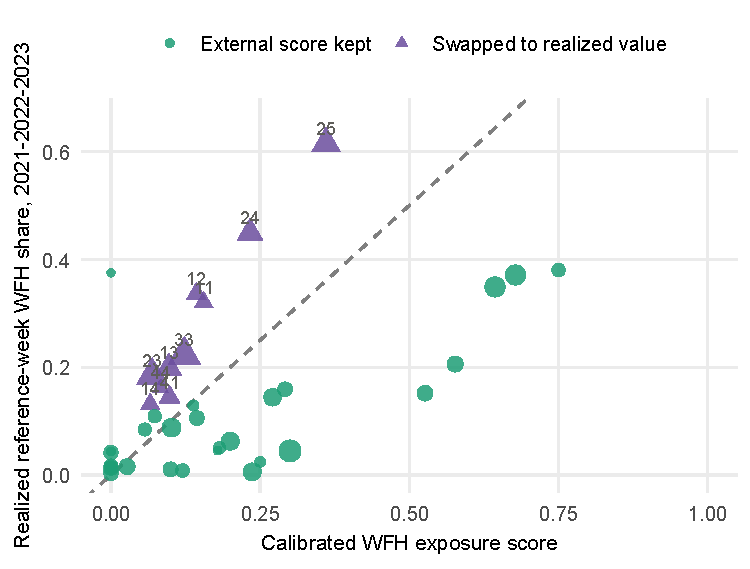
\includegraphics[width=\linewidth]{../outputs/figures/wfh_first_stage_occupation.pdf}\\
{\small (b) Calibrated score against realized reference-week WFH}
\end{minipage}
\caption{Weekly hours by survey year, and the exposure first stage}\label{fig:hours-by-year}
\label{fig:first-stage}
\begin{minipage}{0.95\textwidth}\renewcommand{\baselinestretch}{1}\small
\vspace{0.3em}
\emph{Notes:} Panel~(a): women aged 25--59 who worked in the reference week, unweighted means with
no controls; the upper panel plots each group's mean weekly hours on an axis spanning 36 to 42
hours, the lower panel their difference, with 95\% confidence intervals clustered by individual;
the dotted rule marks the excluded 2020 survey year, and the series break there. Panel~(b): one
point per two-digit occupation, sized by the pooled employed sample in 2021--23; triangles are the
ten occupations the calibration swapped to their realized value, labelled by ISCO-08 code; the
dashed line is the 45-degree line. The swapped occupations sit above it because their calibrated
value is the usual-place share, which is lower than the reference-week share everywhere; the
thirty unswapped ones lie below it, the visual form of the scale-mixing described above.
\end{minipage}
\end{figure}

%======================================================================
\section{The selection correction}\label{sec:app-lee}
%======================================================================

% tables/tab_lee_selection.tex and tables/tab_lee_bounds.tex are still generated by main.R
% (build_paper_tables()) but are no longer input here; the numbers below are quoted from them.
Let $s_{ab} = \Pr(\text{hours observed} \mid \Mother=a, \Post=b)$, the probability of being
employed and working in the reference week. Under parallel trends in selection the
counterfactual for post-period mothers is $s^*_{11} = s_{10} + s_{01} - s_{00}$. If $s_{11}$
exceeds it, the excess share $1 - s^*_{11}/s_{11}$ is trimmed from the $(\Mother=1,\Post=1)$
hours distribution, from the top for the lower bound and from the bottom for the upper bound,
and the model is re-estimated on each trimmed sample. Trimming one tail assumes monotone
selection, and the construction handles only excess selection in that cell. For the DDD the
counterfactual and trim are computed within each quartile of the cell-based exposure index,
which assumes selection depends on exposure only through that quartile, and
equation~\eqref{eq:ddd} is refit on the recombined sample with the occupation-level regressor
and occupation clustering. Because the parameter is partially identified, the
\citet{imbens2004} interval for the identified set is reported with the bounds.

For the DiD, $s_{11} = 0.696$ against $s^*_{11} = 0.683$, and trimming the $1.9\%$ excess gives
bounds of $-0.517$ (SE $0.178$) and $0.802$ (SE $0.179$) around the $0.228$ point estimate,
with Imbens--Manski 95\% interval $[-0.810, 1.096]$. For the DDD the excess is present in all
four quartiles but modest, a trim of $0.80\%$ to $4.48\%$, $1{,}396$ of $72{,}820$ post-period
working mothers; the bounds are $3.126$ (SE $1.144$) and $3.443$ (SE $1.022$) around an
untrimmed $3.232$ (SE $1.054$), which differs from Table~\ref{tab:hours}'s $3.224$ because this
sample additionally requires a matched cell-based exposure, and the Imbens--Manski interval is
$[1.021, 5.324]$.

%======================================================================
\section{Additional results}\label{sec:app-results}
%======================================================================

Figure~\ref{fig:permutation} plots the reference distribution of the permutation test: under the
sharp null the central $95\%$ of cluster-robust $t$-statistics lie between $-2.96$ and $2.60$,
and the observed $3.15$ is exceeded in absolute value by $31$ of $999$ draws.
Table~\ref{tab:extensive} reports the extensive-margin DiD and DDD discussed in
Section~\ref{sec:res-extensive}. Table~\ref{tab:balance-quartile} reports the pre-period
covariate balance between mothers and childless women within each exposure quartile of the hours
DDD's estimation sample, and Figure~\ref{fig:loo} the forty leave-one-occupation-out refits of
the headline estimate.

\begin{figure}[htbp]
\centering
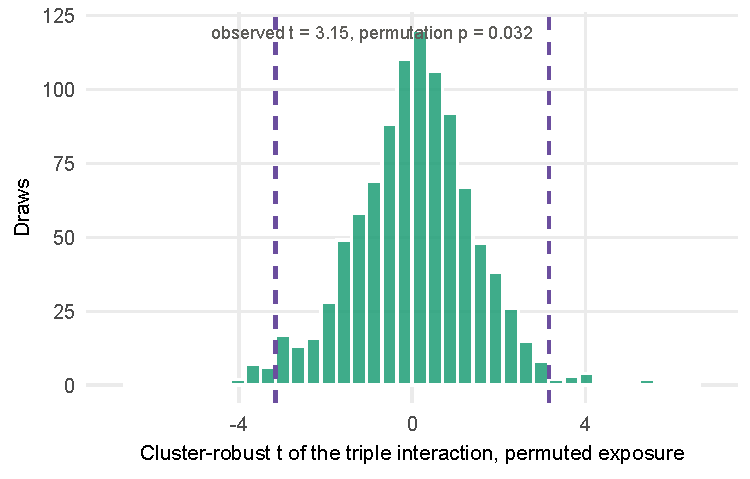
\includegraphics[width=0.55\textwidth]{../outputs/figures/hours_permutation.pdf}
\caption{Permutation distribution of the hours DDD triple interaction}\label{fig:permutation}
\begin{minipage}{0.8\textwidth}\renewcommand{\baselinestretch}{1}\small
\vspace{0.3em}
\emph{Notes:} Histogram of the cluster-robust $t$-statistic of $\Mother \times \Post \times \WFH$
over $999$ random reassignments of the forty exposure scores across occupations, with the same
sample, controls and clustering as column~(2) of Table~\ref{tab:hours}. Dashed lines mark $\pm$
the observed statistic ($3.15$); $p = 0.032$ counts the observed draw \citep{phipson2010}.
\end{minipage}
\end{figure}

\begin{table}[htbp]
\centering
\begin{threeparttable}
\caption{Extensive margin: employment DiD and DDD}\label{tab:extensive}
\renewcommand{\baselinestretch}{1}\scriptsize
\setlength{\tabcolsep}{4pt}
\begin{tabular}{lcc}
\toprule
 & (1) DiD & (2) DDD, cell-based exposure \\
\midrule
Mother $\times$ Post $\times$ WFH\_Exposure &  & $-0.0257$ \\
 &  & $(0.0725)$ \\
Mother $\times$ Post & $-0.0053$ & $0.0065$ \\
 & $(0.0052)$ & $(0.0168)$ \\
Mother $\times$ WFH\_Exposure &  & $-0.1404$\sym{\cdot} \\
 &  & $(0.0803)$ \\
Post $\times$ WFH\_Exposure &  & $-0.1555$\sym{**} \\
 &  & $(0.0566)$ \\
WFH\_Exposure &  & $0.0131$ \\
 &  & $(0.0565)$ \\
Mother & $-0.0034$ &  \\
 & $(0.0041)$ &  \\
Post & $0.0153$\sym{***} &  \\
 & $(0.0043)$ &  \\
Constant & $0.4926$\sym{***} &  \\
 & $(0.0085)$ &  \\
\midrule
MDE ($\alpha=0.05$, power $0.80$), per unit &  & $0.2031$ \\
MDE per SD of exposure &  & $0.0143$ \\
\quad as \% of baseline employment rate &  & 1.85\% \\
\midrule
Observations & 364{,}784 & 355{,}984 \\
$R^2$ & 0.227 & 0.221 \\
Clustering & individual & demographic cell ($\approx 210$) \\
\bottomrule
\end{tabular}

\begin{tablenotes}\footnotesize
\item Dependent variable: employment indicator; full sample of employed and non-employed women;
standard controls in both columns, four decimals because the outcome is a probability. Column (2)
adds Mother $\times$ age-group interactions, so its Mother and Post main effects are not
separately reported, and uses the demographic-cell index of Section~\ref{sec:exposure}, whose
standard deviation on this sample is $0.0706$; the per-SD MDE row is the interpretable one.
Baseline employment rate $0.7737$. \autonoteExtensive
\end{tablenotes}
\end{threeparttable}
\end{table}

\begin{table}[htbp]
\centering
\begin{threeparttable}
\caption{Pre-period covariate balance by quartile of occupation-level WFH exposure}\label{tab:balance-quartile}
\renewcommand{\baselinestretch}{1}\scriptsize
\setlength{\tabcolsep}{4pt}
\begin{tabular}{lcccc}
\toprule
Mothers minus childless women, pre-period & Q1 & Q2 & Q3 & Q4 \\
\midrule
Age-group code (CBS 3--7), mean & $-0.54$\sym{***} & $-0.44$\sym{***} & $-0.33$\sym{***} & $0.08$\sym{*} \\
 & $(0.03)$ & $(0.03)$ & $(0.03)$ & $(0.04)$ \\
Married (\%) & $32.2$\sym{***} & $33.7$\sym{***} & $41.5$\sym{***} & $43.1$\sym{***} \\
 & $(1.1)$ & $(1.1)$ & $(0.9)$ & $(1.3)$ \\
Academic degree (\%) & $10.8$\sym{***} & $4.5$\sym{***} & $1.5$ & $1.8$ \\
 & $(1.2)$ & $(1.2)$ & $(1.0)$ & $(1.2)$ \\
Below high school (\%) & $-3.2$\sym{***} & $-1.7$\sym{***} & $-3.3$\sym{***} & $-0.2$ \\
 & $(0.6)$ & $(0.4)$ & $(0.5)$ & $(0.2)$ \\
Jewish household head (\%) & $1.6$ & $0.5$ & $14.3$\sym{***} & $3.1$\sym{***} \\
 & $(1.0)$ & $(0.7)$ & $(0.9)$ & $(0.8)$ \\
Center or Tel Aviv district (\%) & $-4.4$\sym{***} & $-3.4$\sym{**} & $-8.8$\sym{***} & $-4.5$\sym{**} \\
 & $(1.2)$ & $(1.2)$ & $(1.1)$ & $(1.4)$ \\
Arab (\%) & $1.9$\sym{*} & $0.2$ & $3.7$\sym{***} & $-0.9$ \\
 & $(0.9)$ & $(0.6)$ & $(0.6)$ & $(0.6)$ \\
\midrule
Mothers & 22{,}976 & 24{,}664 & 22{,}562 & 16{,}377 \\
Childless women & 11{,}420 & 11{,}586 & 17{,}244 & 8{,}352 \\
Occupations & 15 & 7 & 11 & 6 \\
Exposure range & 0.00--0.10 & 0.10--0.14 & 0.14--0.30 & 0.36--0.75 \\
\bottomrule
\end{tabular}

\begin{tablenotes}\footnotesize
\item Women working in the reference week in 2017--2019 with a matched two-digit occupation, the
hours DDD's pre-period estimation sample, split into the exposure quartiles of
Figure~\ref{fig:dose-response}. Each cell is the mother-minus-childless difference in the row
variable within the quartile, with a standard error clustered by individual in parentheses;
shares are in percentage points, the age-group code in code units (CBS codes 3--7 span ages
25--59 in five-year bands). Stars follow the paper's legend on a normal reference. Unweighted.
\end{tablenotes}
\end{threeparttable}
\end{table}

\begin{figure}[htbp]
\centering
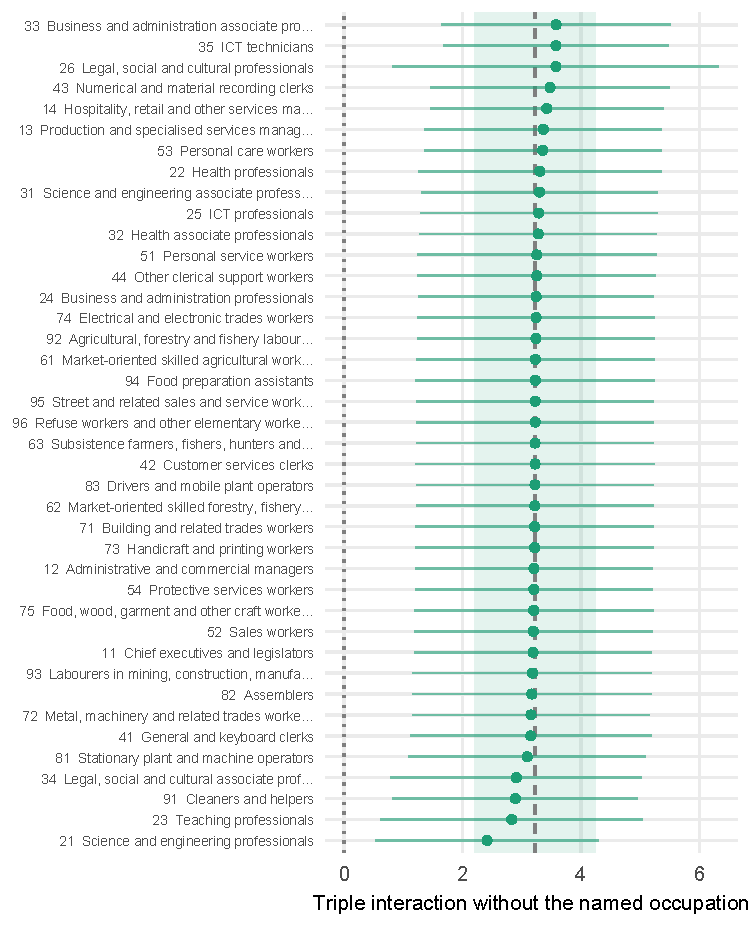
\includegraphics[width=0.75\textwidth]{../outputs/figures/hours_ddd_leave_one_out.pdf}
\caption{Leave-one-occupation-out: the hours DDD triple interaction with each occupation
removed}\label{fig:loo}
\begin{minipage}{0.85\textwidth}\renewcommand{\baselinestretch}{1}\small
\vspace{0.3em}
\emph{Notes:} Each point is $\Mother \times \Post \times \WFH$ from equation~\eqref{eq:ddd}
re-estimated without the occupation named on the axis (column~(2) of Table~\ref{tab:hours} on
39 occupations), with its 95\% confidence interval clustered by occupation; rows are sorted by
the estimate. The dashed line is the headline estimate on all forty occupations and the shaded
band one headline standard error either side of it; the dotted line marks zero. Triangles would
mark refits outside the band; there are none.
\end{minipage}
\end{figure}
